% Built with: bash <skills>/skills/research-paper/scripts/build.sh paper/cheap-world-model
\documentclass[10pt,a4paper]{article}
\usepackage[margin=1in]{geometry}
\usepackage[T1]{fontenc}
\usepackage[utf8]{inputenc}
\usepackage{lmodern}
\usepackage{microtype}
\usepackage{amsmath,amssymb}
\usepackage{booktabs}
\usepackage{graphicx}
\usepackage{xcolor}
\usepackage{caption}
\usepackage{subcaption}
\usepackage{algorithm}
\usepackage{algpseudocode}
\usepackage[hidelinks]{hyperref}
\usepackage{url}
\usepackage[numbers,sort&compress]{natbib}
\usepackage{enumitem}
\usepackage{listings}
\graphicspath{{figures/}}
\setlist{nosep}
\captionsetup{font=small,labelfont=bf}
\lstset{basicstyle=\ttfamily\scriptsize,breaklines=true,breakatwhitespace=false,columns=fullflexible,keepspaces=true,frame=single,framerule=0.3pt}

\newcommand{\ws}{World Sim}
\newcommand{\score}[1]{#1}

\title{\textbf{An Explicit World-Model State for Three Cents:\\ Training-Free Two-View Scene Reconstruction with a Cheap Vision LLM and a Code Sandbox}}
\author{James\\ Independent researcher, San Francisco\\ \texttt{astrojams1@gmail.com}}
\date{September 2026}

\begin{document}
\maketitle

\begin{abstract}
Robot software wants an explicit description of the scene it is acting in---which objects are where, how big, how oriented---and the learned models that provide such descriptions are expensive to train and to run. We ask how cheap an explicit, simulator-ready scene state can get with no training at all. \ws{} sends two uncalibrated photographs of a synthetic room to a low-cost hosted vision model (\texttt{gpt-5-mini}, low reasoning effort) together with a Python sandbox pre-loaded with a 2,000-line classical helper: the helper calibrates both cameras from the room's own silhouette, aligns the two views up to the room's 48 symmetries, detects and triangulates objects, and refines shape, size, position and orientation by rendering hypotheses and comparing them with the photographs. Inside one API call the model runs this loop and returns JSON. On a fixed ten-room benchmark scored with a symmetry-invariant metric, the system reaches a mean of 99.5/100 with six rooms reconstructed exactly, in 22\,s and for \$0.032 per scene (6.3k tokens), and still scores 95.9 with eight objects per room. The result was reached in 26 tuning iterations that moved work out of the model and into deterministic tools: mean score rose from 90.0 to 99.5 while time per scene fell from 232\,s to 22\,s and tokens from 23k to 6k. Running the helper alone, with no language model, reproduces the record scores room for room and scores 99.6 on a held-out set, so on this benchmark the model's contribution is to make a one-call, zero-infrastructure deployment possible rather than to reconstruct anything itself. We release the benchmark, the scorer, the anti-cheating protocol and all 48 benchmark runs, and we state precisely what the benchmark does and does not show.
\end{abstract}

\section{Introduction}

A manipulation or assembly system needs to know the state of the world it is acting on. The dominant answer in learning-based robotics is a \emph{world model}: a learned, action-conditioned predictive model of observations or latents \citep{ha2018world,hafner2019dream,hafner2023mastering,assran2025v,nvidia2025cosmos}. Such models are powerful and expensive: they are trained on large corpora, run on accelerators, and their state is implicit. At the other end of the spectrum sits the oldest answer, an explicit list of objects with poses that a physics engine can simulate directly---what the real-to-sim literature calls a digital twin \citep{dai2024automated,chen2024urdformer,mandi2024real2code}. This paper asks a narrow question about that explicit end: \emph{how cheap can a complete, explicit scene state get if nothing is trained?}

Vision--language models (VLMs) cannot answer this on their own. They fail at elementary geometric perception \citep{rahmanzadehgervi2024vision}, at spatial recall across views \citep{yang2024thinking}, and at multi-view robotic scenes in particular \citep{feng2025seeing}. What they can do is write code, and a recent line of work gives a VLM a Python interpreter with perception and geometry primitives and lets it iterate \citep{gupta2022visual,surs2023vipergpt,hu2024visual,marsili2025visual,cho2026spatialclaw,luo2026pyspatial}. Those systems answer spatial questions. We use the same pattern to produce the state itself, and we measure how much of the result is the model's.

\ws{} (Figure~\ref{fig:feeds}) works as follows. A generator draws a unit-cube room with two to twelve floating red or blue spheres and cubes of three sizes, random wall colors and lighting, and two cameras at unknown positions outside the room, and renders the two camera feeds. The feeds, the fact that the room is a unit cube, the generator's object vocabulary, and a Python sandbox containing \texttt{worldsim.py} are handed to a cheap hosted vision model in a single API call. Nothing else is passed: no camera parameters, no surface colors, no object count. Inside the call the model runs the helper's calibrate--detect--triangulate--render--compare--refine pipeline, reconciles the printout with what it sees, and returns a JSON list of objects. A scorer that is invariant to the room's 48 symmetries and to each cube's 24 rotational symmetries compares the list with the ground truth.

Our findings are as follows. (i) After tuning, the system scores a mean of 99.5/100 on a fixed ten-room benchmark (38 objects), reconstructing six rooms exactly, in 22\,s and \$0.032 per scene, of which \$0.030 is the sandbox session and about \$0.002 is the model; with eight objects per room it scores 95.9 (Section~\ref{sec:results}). (ii) The frontier moved by moving work out of the model: over 26 iterations the mean rose from 90.0 to 99.5 while time fell from 232\,s to 22\,s, tokens from 23k to 6k, and code cells per room from 21.7 to 1.0; the model's reasoning effort could be lowered to \emph{low} once the tool printout was robust (Section~\ref{sec:trajectory}). (iii) The helper alone, run offline with no language model, reproduces the record scores room for room and scores 99.6 on a held-out set; the model's marginal contribution on these rooms is zero (Section~\ref{sec:ablation}). (iv) The remaining errors are what two silhouettes cannot resolve: near-symmetric cube orientations, a coupled position--rotation minimum for an occluded object, and, as rooms get crowded, objects merged into one blob in both views (Section~\ref{sec:failures}).

The contributions are therefore a system and its numbers; a benchmark, a symmetry-invariant metric and an anti-cheating tuning protocol; the tuning trajectory as an empirical study of where accuracy and cost come from in a VLM-plus-tools system; and a failure analysis. We use ``world model'' in the state-estimation sense---an explicit, simulator-ready description of the objects in a scene---rather than the learned latent-dynamics sense of \citet{ha2018world} and \citet{hafner2023mastering}; the resulting scene is a digital twin whose dynamics are supplied by a physics engine, so it complements rather than replaces predictive world models \citep{wang2026world,chen2026definition,ding2024understanding}. All claims are about the synthetic benchmark of Section~\ref{sec:setting}; we make no claim about real photographs.

\begin{figure}[t]
  \centering
  \begin{subfigure}{0.49\linewidth}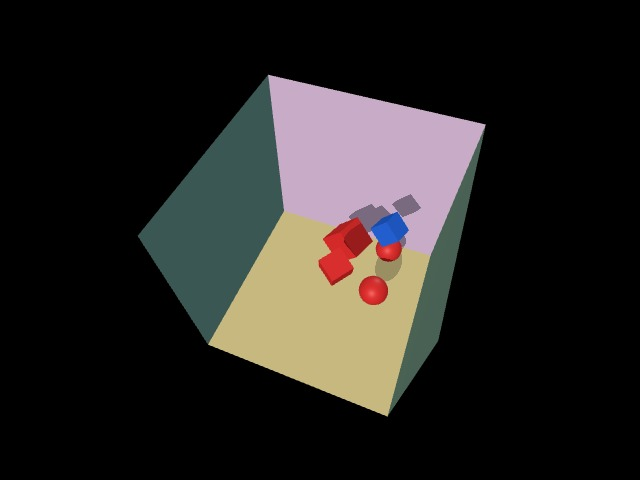
\includegraphics[width=\linewidth]{room101_A.jpg}\caption{Camera A}\end{subfigure}
  \begin{subfigure}{0.49\linewidth}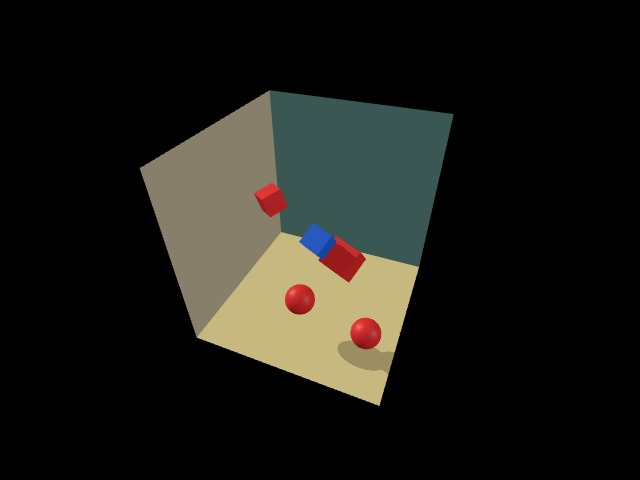
\includegraphics[width=\linewidth]{room101_B.jpg}\caption{Camera B}\end{subfigure}
  \caption{The two feeds the model receives for benchmark room 101 (five objects: two red spheres, two red cubes, one blue cube). The room is seen from outside with its near faces culled; the hexagonal outline is what the helper calibrates the cameras from. The record configuration reconstructs this room at 99.3/100; the single remaining error is one cube centre 0.07 units (1.4 grid steps) off.}
  \label{fig:feeds}
\end{figure}

\section{Related work}

\paragraph{VLM agents with code and tools.}
VisProg \citep{gupta2022visual} and ViperGPT \citep{surs2023vipergpt} showed that an LLM can compose vision modules through generated programs without training. Visual Sketchpad \citep{hu2024visual} adds visual feedback and, unusually, reports per-sample cost (\$0.06--0.13 and 12--27k tokens on GPT-4o). VADAR \citep{marsili2025visual} synthesises a Python API for 3D queries on CLEVR-like scenes and finds, through an oracle experiment, that the vision modules and not the LLM bound accuracy---the decomposition we quantify for reconstruction rather than question answering. SpatialClaw \citep{cho2026spatialclaw} is the closest architecture to ours: a training-free VLM writing cells in a persistent kernel pre-loaded with perception and geometry primitives, with images fed back and a revise loop; pySpatial \citep{luo2026pyspatial}, S-Agent \citep{dai2026s} and Think3D \citep{zhang2026think3d} are multi-view, training-free agents that build a 3D state with learned reconstructors as an intermediate. All of these output answers to questions and none scores the state or reports cost. SpatialBabel \citep{liu20263d} is the closest \emph{task}: VLMs emit executable primitive-scene code (cubes, spheres; position, scale, rotation) from single renders, scored by Hungarian-matched position and scale fidelity, but the code is never executed or compared with the image and positions are ``approximate''. IG-LLM \citep{kulits2024re} is the trained counterpart, fine-tuning an LLM to decode a single CLEVR image into an explicit scene program with a numeric head (L2 position error 0.16--0.21 after 4k training images). We claim none of the ingredients; we claim their closed-loop combination, its measured accuracy--cost--latency frontier, and the finding about where the accuracy comes from.

\paragraph{Analysis by synthesis and inverse graphics.}
Explaining an image by rendering hypotheses and comparing is the classical formulation of vision as inference \citep{yuille2006vision}, made concrete in probabilistic programs \citep{kulkarni2015picture,kulkarni2014inverse}, in learned inverse-graphics networks \citep{kulkarni2015deep}, and in Neural Scene De-rendering \citep{wu2017neural}, whose per-object ``scene XML'' with position and yaw/pitch/roll is the nearest published output format to ours (trained, single view). 3DP3 \citep{gothoskar20213dp3} and Bayes3D \citep{gothoskar2023bayes3d} run render-and-compare in structured generative models---3DP3 even enumerates the cube's 24 rotational symmetries as orientation proposals---but consume depth from a calibrated camera. Our helper is the deterministic, RGB-only, uncalibrated cousin of these systems. CLEVR \citep{johnson2016clevr} defines the primitive-scene universe we borrow, and the object-centric line \citep{burgess2019monet,greff2019multi,locatello2020object,yu2021unsupervised,stelzner2021decomposing} learns to decompose such scenes into masks or latents; none outputs orientation, and all are trained. Training-free 6D pose estimators \citep{wen2023foundationpose,labb2022megapose,caraffa2023freeze} are single-image, per-object and assume known intrinsics.

\paragraph{World models and real-to-sim.}
The term world model dominantly denotes a learned, action-conditioned predictive model \citep{ha2018world,hafner2019dream,hafner2023mastering,assran2025v,nvidia2025cosmos}; \citet{wang2026world} state that a perception module ``is not itself a world model unless it models temporal change'', while \citet{ding2024understanding} and \citet{chen2026definition} recognise an understanding-oriented branch that includes state estimation, and the term is acknowledged to be contested \citep{kong20253d}. Object-centric world models for manipulation \citep{ferraro2023focus,chen2025goal} argue that an explicit object state is the right interface to a policy. On the real-to-sim side, ACDC \citep{dai2024automated} is training-free and VLM-orchestrated but needs a calibrated camera and monocular depth and retrieves assets rather than estimating shape and size (4--16\,cm centre error); URDFormer \citep{chen2024urdformer} and Real2Code \citep{mandi2024real2code} train inverse models from images to URDF/MJCF (Real2Code's zero-shot GPT-4 baseline lost to its fine-tuned model); Agentic Real2Sim \citep{chen2026agentic} confines the VLM to schema-bounded decisions while deterministic geometry tools do the work and reports model bills per episode, the cost convention we follow. SceneScript \citep{avetisyan2024scenescript} and PhysTwin \citep{jiang2025phystwin} are further points on the scene-as-structured-description line. None of these recovers explicit size and orientation of every object from two uncalibrated RGB views with no training and a stated per-scene cost.

\paragraph{Symmetry-aware evaluation.}
BOP's MSSD and MSPD errors \citep{hodan2018bop,hodan2020bop} minimise pose error over an object's symmetry set before comparison; BOP localisation gives the instance count at test time, and BOP 2024 adds a detection task \citep{nguyen2025bop}. Our scorer adopts the symmetry minimisation, adds a scene-level 48-fold symmetry (the room is itself a cube and the cameras are uncalibrated), an explicit assignment between predicted and true object sets, a penalty for extra objects, and joint scoring of discrete attributes with pose.

\section{Problem setting and benchmark}
\label{sec:setting}

\paragraph{Scene state.}
A room is the unit cube $[0,1]^3$ with $y$ up. Its state is a set of objects $S=\{o_1,\dots,o_n\}$, $o_i=(\text{shape}_i,\text{color}_i,s_i,\mathbf{p}_i,R_i)$ with shape $\in\{\text{sphere},\text{cube}\}$, color $\in\{\text{red},\text{blue}\}$, size $s_i\in\{0.10,0.15,0.20\}$ (sphere diameter or cube edge), centre $\mathbf{p}_i\in(0.05\,\mathbb{Z})^3$, and, for cubes, an orientation $R_i\in SO(3)$ given as XYZ Euler angles. The generator (\texttt{src/lib/room.ts}) draws $n\in\{2,\dots,5\}$ by default, or an exact $n\le 12$ on the capacity axis; objects float, keep at least 0.05 from the walls and do not touch; cube orientations are uniform in Euler angles; wall, floor and ceiling colors are muted hues kept away from red and blue; one shadow-casting distant light, an ambient term and a fill light are drawn at random. Two cameras sit on a sphere of radius 1.7--2.6 around the room centre at 25--60$^\circ$ elevation, at least 50$^\circ$ apart in azimuth, with a field of view just containing the room, and look near the centre. Everything is a deterministic function of a seed.

\paragraph{Observation.}
Each camera renders a $640\times480$ JPEG with three.js. Because the camera is outside the room the near faces are culled, so the feed shows the room as an open box on black whose outline is a hexagon of six room corners (Figure~\ref{fig:feeds}). The system receives the two JPEGs, the statement that they are two views of a $1\times1\times1$ room from unknown viewpoints outside it, the object vocabulary above (including ``between 2 and 12 objects''), the output schema, and the helper module. It is denied camera intrinsics and extrinsics, surface colors, the object count and the seed. A static check forbids the server route from touching any room or camera data, and the benchmark driver intercepts every request to verify that its body contains only the model name, the reasoning effort and the two image data URLs exactly as displayed on the page.

\paragraph{Score.}
Let $G$ be the 48-element symmetry group of the cube, acting on positions and orientations. Because nothing marks which corner is the origin, a prediction $\hat S$ is compared with the truth $S$ under the best $g\in G$:
\begin{equation}
\mathrm{score}(\hat S,S)=\max_{g\in G}\;\max_{\pi}\;\frac{100}{|S|}\Big[\sum_{i\,\text{matched}} c\big(g\cdot\hat o_{\pi(i)},\,o_i\big)\;-\;\#\text{extra}\Big],
\label{eq:score}
\end{equation}
where $\pi$ ranges over injective assignments of true objects to predicted ones (exhaustive), an unmatched true object scores 0, each unmatched prediction costs as much as a missing object, and the per-object credit $c\in[0,1]$ awards 0.2 for the correct shape, 0.2 for color, 0.2 for size within 0.012, and 0.4 for position within 0.03 (spheres) or 0.3 for position plus 0.1 for orientation within $10^\circ$ (cubes); position and size credit decay linearly to zero at 0.35 and orientation credit at $45^\circ$. Orientation error is the rotation angle between $\hat R$ and $R$ minimised over the cube's 24 rotational symmetries. A room scores 100 only when every object is matched within tolerance with no extras (``exact'').

\paragraph{Benchmark protocol.}
The benchmark is seeds 101--110 with the default draw (38 objects: 2--5 per room). Seeds 201--210 are a held-out set used only offline (Section~\ref{sec:ablation}) and never for a record decision. The capacity axis renders the same seeds with exactly $n\in\{6,8,10,12\}$ objects; capacity is the largest $n$ at which the two-run mean is at least 95. A tuning iteration is one hypothesis and one change to the prompt or the helper; a candidate record must be confirmed by a second run of the same configuration, and the record is the mean of both. A new record requires $+1.0$ mean score, or an equal score (within 1.0) with 20\,\% lower cost or 30\,\% lower time per room. Runs that fail with an API-side error (rate limit, moderation false positive) are retried once; timeouts and wrong answers are never retried. Reported time is wall-clock per room with three rooms in flight; tokens are the API's usage counts; cost is list price plus \$0.03 for one code-interpreter session per room (the sandbox price at the time of the runs).

\section{System}
\label{sec:system}

\paragraph{One call.}
The server uploads \texttt{camera\_A.jpg}, \texttt{camera\_B.jpg} and \texttt{worldsim.py} to a code-interpreter container and starts one background response with the system prompt (Appendix~\ref{app:prompt}), the two images as inputs, the \texttt{code\_interpreter} tool and a JSON schema for the answer; the client polls. The prompt states the vocabulary, the helper's API, and a five-step method: look at both images and count objects and colors; run the whole pipeline in one cell; reconcile the printout with the visual inventory, touching only what eyes can judge better than silhouettes (add an object merged into a shared blob, remove a phantom, fix a color; never edit numbers); re-verify if anything changed; output the printed JSON verbatim. Everything the model prints in the sandbox is teed into a transcript file that the server fetches from the container afterwards.

\paragraph{Self-calibration from the room silhouette.}
The helper thresholds the non-black region of each feed, traces its contour and simplifies it to a hexagon of six pixel corners $\mathbf{u}_1..\mathbf{u}_6$. Each corner is one of the eight cube vertices, and the visible hexagon admits a small set of consistent labellings, which differ from one another only by a symmetry in $G$. For each labelling the helper fits a pose $(R,\mathbf{t})$ and focal length $f$ by least squares on the reprojection error
\begin{equation}
E(R,\mathbf{t},f)=\sum_{k=1}^{6}\big\|\Pi_f(R\,\mathbf{X}_{\ell(k)}+\mathbf{t})-\mathbf{u}_k\big\|^2 ,
\label{eq:pose}
\end{equation}
where $\mathbf{X}_{\ell(k)}$ is the cube vertex assigned to corner $k$ and $\Pi_f$ the pinhole projection with unknown $f$. A DLT initialisation is refined first; if it does not reach 1\,px, a batch of random rotation starts over five fields of view is solved at once, and the first labelling that fits within 1\,px is accepted. When the hexagon is degenerate (a true pentagon: one corner collinear with two others) or two corners nearly coincide, alternative outlines---merged, coarser, five-corner---are tried, the five-point case with 600 random starts since no closed-form initialisation exists. Over the 40 benchmark and held-out cameras the accepted fits are all under 1.5\,px.

\paragraph{Frame alignment.}
Camera B's pose is expressed in camera A's frame by scoring all 48 candidate transformations: the colors of the room faces visible in both images must agree, and the rays of same-colored blobs must nearly intersect. Near-ties are broken by image fit. The prompt does not need to know which frame was chosen; the scorer is invariant to it.

\paragraph{Detection, matching, hypothesis.}
Red and blue masks require the dominant channel to exceed the others by 45 (so bluish-grey walls are not blobs); connected components of at least 150 pixels become blobs with area, bounding box, centroid and circularity. Blobs are paired across the views by an assignment that minimises ray gap plus a term for the mismatch between the sizes implied by each blob's width, capped at the six largest blobs per color. Each pair yields an object: triangulated centre, size from apparent width, and an initial shape from circularity. A blob paired in only one view is explained by a search along its ray over depth and, for cubes, rotation, scored with a depth buffer so that the part of a candidate hidden behind nearer objects is neutral and the visible part must land on unexplained pixels of its color.

\paragraph{Analysis by synthesis.}
Every subsequent decision is made by rendering. For an object $o$ and view $v$, $\mathrm{cov}_v(o)$ is its soft (3$\times$ super-sampled) silhouette and $M_v$ the real mask of its color with the other objects' renders subtracted; the per-object objective is $J(o)=\sum_v \mathrm{IoU}\big(\mathrm{cov}_v(o),M_v\big)$, skipping a view in which the object is more than half hidden. Coordinate descent over position on the grid, size over the three legal values and, for cubes, orientation maximises $J$ for each object in turn; orientation is refined with 150 random starts for every legal size so that a cube seen one size too large cannot settle into a wrong orientation. Sphere versus cube is decided by fitting the object both ways: a cube, having free size and rotation, must win by a margin (0.06 IoU, halved for the smallest size) since it can mimic a disc; when silhouettes are inconclusive the fraction of flat-gradient pixels inside the blob (flat faces with edges versus one smooth gradient, with size-specific thresholds measured on 130 blobs) casts the vote. A blob shared with another object in one view is judged from the other view alone; a blob shared in both views is left alone. Finally \texttt{compare} renders the hypothesis in both views and reports mean IoU, per-object pixel offsets, phantoms (objects whose footprint falls on too few real pixels of their color) and unexplained real blobs. Algorithm~\ref{alg:solve} lists the one-call pipeline.

\begin{algorithm}[t]
\caption{\texttt{solve\_all}: the helper's automatic pipeline (no model in the loop)}
\label{alg:solve}
\begin{algorithmic}[1]
\State outlines $\gets$ room silhouettes of A and B, simplified to hexagons (with pentagon/merged fallbacks)
\State $(R_A,\mathbf{t}_A,f_A),(R_B,\mathbf{t}_B,f_B)\gets$ first corner labelling whose least-squares fit of Eq.~\eqref{eq:pose} is within 1\,px
\State $R_B,\mathbf{t}_B\gets$ best of the 48 room symmetries by face colors and blob triangulation
\State blobs $\gets$ red/blue connected components in each view; matches $\gets$ assignment by ray gap and apparent size
\State objects $\gets$ one object per match (triangulated centre, size from width, shape from circularity); 3 passes of coordinate descent
\State objects $\gets$ objects $\cup$ objects explaining unpaired blobs along their rays (depth-buffered)
\State shapes $\gets$ sphere-vs-cube fit with margin and shading vote; apply; coordinate descent over position/size/orientation
\State orientations $\gets$ random-start refinement for every legal size; settle positions if a size changed
\State report $\gets$ render both views, compare with the images (IoU, offsets, phantoms, unexplained blobs)
\State print report and answer JSON under a banner: \textsc{final} if no open issue, else the one thing to fix
\end{algorithmic}
\end{algorithm}

\paragraph{What is left to the model.}
The prompt reserves for the model's eyes the object count and colors, the splitting of a blob that contains two touching objects (via \texttt{object\_from\_pixels} with pixel centres it reads off the images), the removal of phantoms, and the decision to stop. Shape verdicts are final unless the model sees straight edges in both images; numbers are never typed. \texttt{finish} re-verifies after any change and prints the answer under a \textsc{final answer} banner when no issue is open, or when the open issue is identical to the previous call's (two views cannot resolve it). The model is told that running any further cell after \textsc{final} is an error. In the record configuration nine of ten rooms finish in one cell and the tenth in two.

\section{Results}
\label{sec:results}

\paragraph{Record configuration.}
Table~\ref{tab:record} lists the two confirming runs of the record configuration (iteration 23 of Section~\ref{sec:trajectory}). The two-run mean is \score{99.5}/100 with six rooms exact in each run; per-room scores are identical across the two runs. Per room, wall-clock time is 17--31\,s (mean 22.3\,s over both runs, 115 and 134\,s of wall clock for ten rooms with three in flight), tokens 5.5--6.8k (mean 6,274), and estimated cost \$0.032. The 38 objects are all matched with the right shape, color and size; the four remaining errors are one sphere centre 0.071 off (room 101), two cube orientations off by $11^\circ$ and $41^\circ$ (rooms 104, 105), and a cube in room 108 that is hidden behind a sphere in camera B and lands one grid step deep with an $18^\circ$ orientation error.

\begin{table}[t]
\centering\small
\caption{Record configuration (\texttt{gpt-5-mini}, reasoning effort \emph{low}, iteration 23), seeds 101--110, two runs. Time is wall clock per room with three rooms in flight; tokens are the API's total (input incl.\ cached, output incl.\ reasoning) for run 2. Remaining errors are attribute errors beyond tolerance under the best assignment and room symmetry.}
\label{tab:record}
\begin{tabular}{@{}rrrrrrl@{}}
\toprule
Room & Objects & Score (run 1) & Score (run 2) & s & Tokens & Remaining error (run 2) \\
\midrule
101 & 5 & 99.3 & 99.3 & 28 & 6,832 & pos 0.071 \\
102 & 3 & 100.0 & 100.0 & 17 & 5,752 & — \\
103 & 3 & 100.0 & 100.0 & 18 & 5,930 & — \\
104 & 5 & 99.9 & 99.9 & 31 & 6,646 & ori 11° \\
105 & 3 & 97.0 & 97.0 & 19 & 5,997 & ori 41° \\
106 & 3 & 100.0 & 100.0 & 23 & 5,817 & — \\
107 & 5 & 100.0 & 100.0 & 31 & 6,690 & — \\
108 & 4 & 98.6 & 98.6 & 23 & 6,349 & pos 0.071; ori 18° \\
109 & 5 & 100.0 & 100.0 & 21 & 6,512 & — \\
110 & 2 & 100.0 & 100.0 & 21 & 5,475 & — \\
\bottomrule
\end{tabular}

\end{table}

\paragraph{Cost and latency anatomy.}
Of the \$0.032 per room, \$0.030 is the flat code-interpreter session price; the model's tokens cost about \$0.002 (run 2 mean: 5,783 input tokens of which 2,726 cached, 417 output tokens of which 147 are reasoning, at list prices of \$0.25/\$0.025/\$2.00 per million). The cost floor of this design is therefore the sandbox, not the model, and cost records were effectively closed from iteration 3 onwards; time and accuracy were the remaining levers. Of the roughly 22\,s per room, the helper's own computation takes 3--10\,s in the sandbox (it is 2--3$\times$ slower there than on a laptop), and the rest is fixed API overhead and the model turn; by the end of tuning the per-room time was dominated by that fixed part.

\paragraph{Capacity.}
Table~\ref{tab:capacity} reports the capacity ladder with the model in the loop, and Table~\ref{tab:capacity_offline} and Figure~\ref{fig:capacity} the same rooms with the pipeline alone. With six objects per room the configuration scores 97.7 and with eight 95.9 (two confirming runs, identical per-room scores), so the capacity record is eight objects; with ten it falls to 89.5 and the pipeline alone reaches 80.8 with twelve. The losses change character as rooms fill: at eight objects one object is lost and the rest are orientation and one-grid-step errors on crowded cubes; at ten, five objects are missing across the ten rooms; at twelve, thirteen. A missing object is one that overlaps another of its color in \emph{both} views, so that each view shows a single blob; the helper explains a blob seen unpaired in one view along its ray from the other, but a cluster merged in both views leaves no unexplained pixels to search for (Section~\ref{sec:failures}).

\begin{table}[t]
\centering\small
\caption{Capacity axis: seeds 101--110 rendered with an exact object count. Capacity is the largest count whose two-run mean reaches 95; \texttt{capacity-6} and \texttt{capacity-8} predate the frame tie-breaker and tighter pairing of the final helper, \texttt{-b} and \texttt{-confirm} use it.}
\label{tab:capacity}
\begin{tabular}{@{}rlrrrrr@{}}
\toprule
Objects & Run & Mean & Exact & s/room & Tokens & \$/room \\
\midrule
6 & capacity-6 & 94.2 & 3 & 33 & 7,837 & 0.033 \\
6 & capacity-6-b & 97.7 & 3 & 28 & 7,917 & 0.033 \\
8 & capacity-8 & 93.2 & 2 & 31 & 8,276 & 0.033 \\
8 & capacity-8-b & 95.9 & 3 & 29 & 8,821 & 0.033 \\
8 & capacity-8-confirm & 95.9 & 3 & 29 & 8,313 & 0.033 \\
10 & capacity-10 & 89.5 & 1 & 35 & 9,391 & 0.033 \\
\bottomrule
\end{tabular}

\end{table}

\begin{table}[t]
\centering\small
\caption{Capacity axis, pipeline alone (offline, no model) on the same rooms, with the model-in-the-loop means of Table~\ref{tab:capacity} for comparison (the six-object entry is the \texttt{-b} run, which uses the final helper). ``Missing'' counts true objects left unmatched over the ten rooms. Offline seconds are on two vCPUs.}
\label{tab:capacity_offline}
\begin{tabular}{@{}rrrrrr@{}}
\toprule
Objects & Pipeline mean & Exact & Missing objects & s/room (offline) & LLM + tools mean (two-run) \\
\midrule
6 & 97.3 & 3 & 0 & 8 & 97.7 \\
8 & 95.9 & 3 & 1 & 10 & 95.9 \\
10 & 90.4 & 1 & 5 & 13 & 89.5 \\
12 & 80.8 & 0 & 13 & 14 & — \\
\bottomrule
\end{tabular}

\end{table}

\begin{figure}[t]
  \centering
  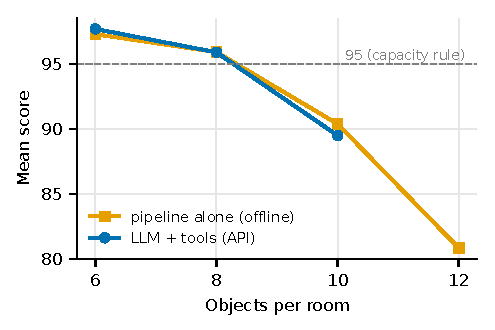
\includegraphics[width=0.55\linewidth]{capacity.pdf}
  \caption{Mean score against objects per room for the pipeline alone (offline, 6--12 objects) and with the model in the loop (API, 6--10 objects). The two coincide within run noise; the capacity rule's threshold of 95 is passed at eight objects.}
  \label{fig:capacity}
\end{figure}

\section{Pipeline alone versus model plus pipeline}
\label{sec:ablation}

The natural ablation is to remove the language model. We rendered the benchmark and held-out rooms with the app (no API involved), ran \texttt{solve\_all} on the two JPEGs offline with the same helper file, and scored the printed JSON with the same scorer. Table~\ref{tab:ablation} compares this with the record run. On all ten benchmark rooms the pipeline alone returns the same score as the model-in-the-loop run---to the decimal---because in the record configuration the model runs one cell and outputs the printout verbatim; its visual reconciliation step never fires. On the held-out rooms 201--210, which no tuning decision was ever based on with the API and which were only ever used to reject helper changes that hurt them offline, the pipeline alone scores 99.6 with seven rooms exact (Table~\ref{tab:heldout}); the three misses are again a cube orientation and two centres within two grid steps.

\begin{table}[t]
\centering\small
\caption{Removing the model. ``Pipeline alone'' runs the helper's \texttt{solve\_all} on the same two JPEGs with no language model; ``LLM + tools'' is run 2 of the record configuration. Offline time on two vCPUs, with other jobs running, is 8--21\,s per room and is not comparable to the sandbox.}
\label{tab:ablation}
\begin{tabular}{@{}rrrrl@{}}
\toprule
Room & Objects & LLM + tools (run 2) & Pipeline alone & Difference \\
\midrule
101 & 5 & 99.3 & 99.3 & identical \\
102 & 3 & 100.0 & 100.0 & identical \\
103 & 3 & 100.0 & 100.0 & identical \\
104 & 5 & 99.9 & 99.9 & identical \\
105 & 3 & 97.0 & 97.0 & identical \\
106 & 3 & 100.0 & 100.0 & identical \\
107 & 5 & 100.0 & 100.0 & identical \\
108 & 4 & 98.6 & 98.6 & identical \\
109 & 5 & 100.0 & 100.0 & identical \\
110 & 2 & 100.0 & 100.0 & identical \\
\midrule
mean & 38 & 99.5 & 99.5 & \\
\bottomrule
\end{tabular}

\end{table}

\begin{table}[t]
\centering\small
\caption{Held-out seeds 201--210, pipeline alone (the API was never run on these rooms).}
\label{tab:heldout}
\begin{tabular}{@{}rrrl@{}}
\toprule
Room & Objects & Helper alone & Remaining error \\
\midrule
201 & 5 & 100.0 & — \\
202 & 2 & 100.0 & — \\
203 & 3 & 100.0 & — \\
204 & 5 & 98.2 & pos 0.071; ori 16°; ori 23° \\
205 & 5 & 99.1 & pos 0.071 \\
206 & 4 & 100.0 & — \\
207 & 2 & 100.0 & — \\
208 & 3 & 100.0 & — \\
209 & 5 & 100.0 & — \\
210 & 4 & 98.8 & ori 15°; pos 0.071 \\
\midrule
mean / total & 38 & 99.6 & 7 of 10 rooms exact \\
\bottomrule
\end{tabular}

\end{table}

This is the paper's central honesty point and we state it plainly: \emph{on this benchmark the reconstruction is done by 2,000 lines of classical geometry, and the model's marginal contribution to accuracy is zero.} It was not always zero. Early in tuning the model's reconciliation step mattered---iteration 12 added a rule that the object count must never drop below the visual count after the low-effort model had deleted real objects, and transcripts of iterations 2--8 show the model adding merged objects and removing phantoms---but each such intervention was a signal that the helper should do it deterministically, and by iteration 19 it did. What remains of the model is the harness: a single API call that needs no GPU, no server-side Python environment and no per-scene engineering, at a price set by the sandbox. Whether a model ever helps on rooms the helper fails---the capacity rooms with blobs merged in both views---is the experiment we did not run (Section~\ref{sec:recommended}). The capacity ladder gives a hint: at eight and ten objects the model-in-the-loop runs are again identical room for room to the pipeline (``the model copies the pipeline'', in the benchmark log), so the model did not split the merged blobs either.

\section{How the frontier moved}
\label{sec:trajectory}

The 26 tuning iterations were carried out in eleven hours on 2026-09-05 by an AI coding agent following a written procedure (Appendix~\ref{app:protocol}): read the benchmark log, state one hypothesis, change the prompt or the helper, run the ten rooms, append a row to the log whether or not it is a record, confirm candidates with a second run, and never touch the scorer, the generator or the seeds. The 48 result files (454 room solves, 5.1\,M tokens, \$16.07 of API spend, one API-side error, zero anti-cheat violations) are in the repository. Figure~\ref{fig:frontier} plots them; Table~\ref{tab:history} in the appendix lists every iteration.

\begin{figure}[t]
  \centering
  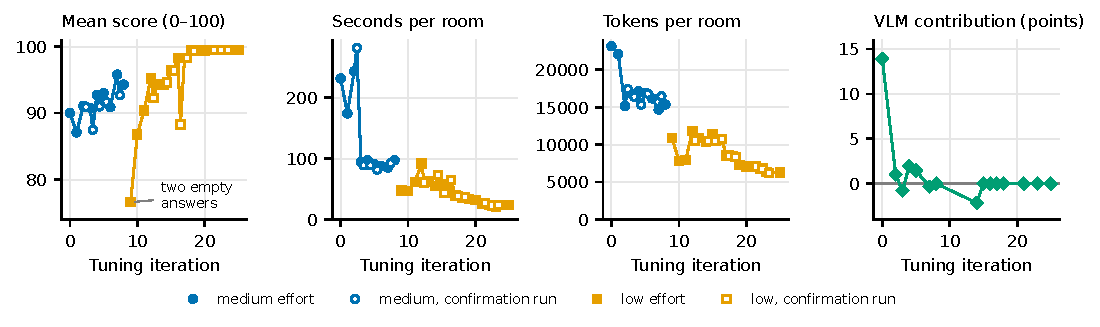
\includegraphics[width=\linewidth]{frontier.pdf}
  \caption{The tuning trajectory: mean score, seconds and tokens per room for every benchmark run (candidate and confirmation runs both shown; $x$ offset marks confirmations). Iterations 0--8 used medium reasoning effort, 9--25 low. The score dip at iteration 9 is two rooms answered with an empty object list after the low-effort model lost a truncated printout.}
  \label{fig:frontier}
\end{figure}

\paragraph{Work moved from the model to the tools.}
The baseline (iteration 0) already contained the helper's primitives and scored 90.0, but the model orchestrated them itself in 21.7 code cells per room over 232\,s and 23k tokens. Iteration 2 folded the whole pipeline into one \texttt{solve\_all} call and cut tokens by 30\,\%; iteration 4 forbade the model from editing numbers and told it to output the printout verbatim; iterations 7, 16, 17 and 18 moved the shape decision, the size--rotation coupling, the phantom test and occlusion handling into the helper, each time removing a class of model intervention; iteration 19 let \texttt{solve\_all} print the final banner so that nine rooms finish in one cell; iterations 20--23 then cut sandbox compute and printout length. Score, time and tokens improved together: every record after iteration 7 was either a score gain with a time gain or a pure time/token gain at equal score.

\paragraph{Reasoning effort.}
Iteration 9 ran the iteration-8 code with the model's reasoning effort lowered from medium to low. Eight rooms scored exactly as before at half the time and 30\,\% fewer tokens, but two rooms returned an empty object list: transcripts showed that the bootstrap's \texttt{help(ws)} printed 15k characters, the sandbox truncated the output, and the low-effort model then ``could not see'' the report and gave up after 10--13 cells. Excluding the two empty answers the low-effort mean was 95.8 against 94.3 for medium. Removing the long printout and adding a fallback rule fixed the failure, and every later record is at low effort. The lesson generalises: a weaker reasoning setting does not reason worse on this task, it copes worse with broken tool output, and robustness of the tool printout is what unlocks the cheaper setting.

\paragraph{Run-to-run variance.}
Fourteen configurations were run twice. Across the 139 room pairs (one API error excluded), 84\,\% of rooms scored identically in both runs, the median absolute difference is 0 and the 90th percentile 7 points; the largest single-room difference is 27 points (iteration 12) and the largest difference between two runs' means 10.0 points, in iteration 16's confirmation, where one room's request was rejected by a moderation false positive and counted as zero. At the record, all ten rooms are identical across the two runs. Variance therefore shrank with the number of code cells: once the model runs one deterministic cell, the run is deterministic up to API errors, which is why a second confirming run is cheap insurance early in tuning and a formality at the end.

\paragraph{Negative results.}
Two offline attempts were reverted. A second rotation-refinement pass after a position pass (iteration 24) left the two coupled-minimum rooms unchanged and worsened room 105 from $41^\circ$ to $52^\circ$; scoring the true orientation in the solver's frame showed that rooms 104 and 105 are true silhouette ambiguities (the true rotation scores the same overlap as the found one), while room 108 is a coupled position--rotation local minimum (true pose 0.92--0.96 versus 0.68--0.79). Explaining unexplained residual regions of a color along their rays (iteration 26, aimed at capacity) gained 0.1--1.1 points at eight and twelve objects but produced phantom objects on the held-out set (99.6 $\to$ 87.4) and was not adopted, because the protocol forbids lowering the default sets to gain capacity.

\section{Failure analysis}
\label{sec:failures}

At the record the errors are of three kinds, and all three are limits of two silhouettes rather than of the search. (1) \emph{Silhouette-ambiguous orientation}: a cube whose two silhouettes are equally well explained by two orientations $11^\circ$ and $41^\circ$ apart (rooms 104 and 105); the true rotation scores no better than the found one, so no silhouette-based objective can recover it, and only shading or a third view could. (2) \emph{Coupled position--rotation minimum for an occluded object}: room 108's blue cube is hidden behind a blue sphere in camera B, so its depth is constrained by one view only and the search settles one grid step deep with a compensating rotation; a shading term or a contact prior would be the remedy. (3) \emph{A single grid step}: room 101's sphere centre 0.071 off after a size change, within the search's local basin. As the object count rises the dominant failure changes: objects of the same color that overlap in \emph{both} views form one blob in each and are reconstructed as one object; the helper's residual-region search can find them only at the price of phantoms elsewhere (iteration 26), and the model, in the runs we have, did not split them either. Two of about 450 requests were rejected by the provider's moderation on an unchanged prompt; the benchmark retries such API-side errors once and reports them.

\section{Limitations}
\label{sec:limitations}

The benchmark is synthetic, with two colors, two shapes, three sizes, a grid of positions, a unit room with a clean black background, and at most twelve objects; the helper's silhouette calibration and color masks exploit every one of these facts, and nothing here transfers to a photograph without new tools. The record is on ten rooms that the tuning loop optimised against; the held-out set guards against overfitting but was only ever run offline, so an API run on it is owed (Section~\ref{sec:recommended}). ``Training-free'' means that no component was trained by us; the vision model is trained, and the shading thresholds were measured on 130 blobs from the same generator. One model from one provider was used; the effort ablation is on ten rooms. Cost figures are list prices on the day of the runs, and the \$0.030 sandbox session that dominates them is a pricing decision, not a property of the method. There are no dynamics: the output is a state, and any world model in the predictive sense has to be built on top of it by a simulator.

\section{Recommended experiments}
\label{sec:recommended}

Each of the following is a single command in the repository and costs about \$0.32 per ten-room run. (i) The API on the held-out seeds 201--210 (\texttt{--seeds 201,\dots,210}), to report a model-in-the-loop number that no tuning decision touched. (ii) The model without the sandbox, and the model with a sandbox but without \texttt{worldsim.py}, as the two VLM-only baselines; the repository records that \texttt{gpt-4.1-mini} sometimes answers without running code, and that number should be measured rather than described. (iii) Capacity rooms where the model is asked to split blobs the pipeline reports as too wide, to test whether a model ever adds accuracy where the tools fail. (iv) Other cheap models (\texttt{gpt-5-nano}, \texttt{gpt-4o-mini}) at the record prompt, to separate the harness from the model. (v) A physical unit-cube room with painted spheres and cubes and two phone cameras, as the smallest possible step toward real images.

\section{Conclusion}

A cheap vision model given a code sandbox and a classical, self-calibrating analysis-by-synthesis helper recovers the complete explicit state of a synthetic two-view scene at 99.5/100, in 22\,s and for about three cents, with no training; the accuracy was obtained by moving work from the model into deterministic tools, and the model's marginal contribution to accuracy on the benchmark is zero. We think the negative half of that sentence is as useful as the positive half: for explicit scene state on structured scenes, the cheapest world model without training is a good tool library and a model that knows when to call it once.

\paragraph{Reproducibility.}
Code, prompt, helper, scorer, benchmark driver, anti-cheat check and all 48 result files: \url{https://github.com/astrojams1/world-sim} (commit \texttt{d3b8a2d}). The offline ablation, the analysis scripts and this paper's source are under \texttt{paper/cheap-world-model/} in the same repository; every table and figure is generated from the result files by \texttt{scripts/analyze\_bench.py}.

\paragraph{Disclosure.}
The system, its 26 tuning iterations and the text of this paper were produced with AI coding agents (Claude) directed by the author, who set the task, the anti-cheating rules and the claims and is responsible for the content. The benchmarked model is \texttt{gpt-5-mini} accessed through the OpenAI Responses API.

\bibliographystyle{plainnat}
\bibliography{refs}

\appendix

\section{The system prompt}
\label{app:prompt}
The prompt is generated by \texttt{src/lib/skill.ts}; sizes and grid are substituted from the generator's constants. It is reproduced verbatim.
\lstinputlisting{experiments/system-prompt.txt}

\section{Tuning protocol}
\label{app:protocol}
The agent-facing procedure is \texttt{.claude/skills/tune-skill/SKILL.md} in the repository. Its ground rules: the model receives only the two unaltered images, the unit-cube statement, the object rules and the output format; only the prompt, the helper, the model and effort defaults and the request plumbing may change; the scorer, generator and seed set may not; every run must pass the static no-cheating check and the runtime request check; API-side errors are retried once and reported, wrong answers never; one hypothesis per iteration, a row in the log regardless of outcome, a confirming second run for candidates, and a held-out offline check for helper changes that are neutral on the benchmark.

\section{All benchmark runs}
\begin{table}[h]
\centering\scriptsize
\caption{Every benchmark run in \texttt{bench/results/}, in order. Cells is the mean number of code-interpreter calls per room. Iteration 24 and 26 were offline-only and are not in the table; capacity runs are in Table~\ref{tab:capacity}.}
\label{tab:history}
\begin{tabular}{@{}rlp{5.6cm}rrrrrr@{}}
\toprule
It. & Effort & Change tested & Mean & Exact & s/room & Tokens & \$/room & Cells \\
\midrule
0 & medium & baseline prompt + helper, medium effort & 90.0 & 2 & 232 & 23,132 & 0.045 & 21.7 \\
1 & medium & silhouette shape check in prompt; soft renders & 87.1 & 3 & 174 & 22,089 & 0.044 & 20.3 \\
2 & medium & one-shot solve\_all pipeline + finish() & 91.1 & 3 & 243 & 15,160 & 0.038 & 11.3 \\
2 & medium & \emph{confirmation run} & 90.9 & 3 & 282 & 17,429 & 0.040 & 16.6 \\
3 & medium & per-object search on residuals; blob caps & 90.8 & 4 & 95 & 16,809 & 0.040 & 11.9 \\
3 & medium & \emph{confirmation run} & 87.5 & 4 & 89 & 16,373 & 0.040 & 13.6 \\
4 & medium & shape verdicts final; output JSON verbatim; 6-cell cap & 92.7 & 5 & 97 & 17,128 & 0.040 & 14.1 \\
4 & medium & \emph{confirmation run} & 91.0 & 4 & 89 & 15,339 & 0.039 & 13.2 \\
5 & medium & grid-aligned wall margin; size-scaled cube margin & 93.0 & 3 & 91 & 16,886 & 0.040 & 14.1 \\
5 & medium & \emph{confirmation run} & 91.7 & 2 & 82 & 16,814 & 0.040 & 12.8 \\
6 & medium & FINAL ANSWER banner as hard stop & 90.9 & 2 & 87 & 16,173 & 0.040 & 11.6 \\
7 & medium & shading tie-break for sphere vs cube & 95.8 & 4 & 85 & 14,680 & 0.038 & 10.0 \\
7 & medium & \emph{confirmation run} & 92.7 & 3 & 92 & 16,453 & 0.040 & 13.8 \\
8 & medium & apparent-size term in blob pairing & 94.3 & 3 & 97 & 15,368 & 0.039 & 11.4 \\
9 & low & same code, reasoning effort low & 76.6 & 3 & 48 & 10,845 & 0.034 & 7.2 \\
10 & low & truncation fallback; no help(ws); outline de-dup & 86.8 & 4 & 47 & 7,803 & 0.033 & 2.5 \\
11 & low & candidate outlines (6/5-corner fallbacks) & 90.4 & 3 & 62 & 7,923 & 0.034 & 2.8 \\
12 & low & transcript tee moved into helper; count rule & 95.2 & 3 & 92 & 11,828 & 0.036 & 4.3 \\
12 & low & \emph{confirmation run} & 92.3 & 3 & 61 & 10,560 & 0.035 & 3.0 \\
13 & low & capped outline fallback & 94.3 & 3 & 62 & 10,856 & 0.035 & 3.0 \\
14 & low & five-corner (pentagon) outline fit & 94.3 & 3 & 55 & 10,422 & 0.035 & 2.6 \\
14 & low & \emph{confirmation run} & 94.6 & 4 & 73 & 10,508 & 0.035 & 3.0 \\
15 & low & batched pose fit; early stop; app default low & 96.4 & 5 & 58 & 11,442 & 0.035 & 3.8 \\
15 & low & \emph{confirmation run} & 96.4 & 5 & 44 & 10,534 & 0.035 & 3.0 \\
16 & low & size+rotation joint refine; chroma masks; overlap test & 98.3 & 7 & 55 & 10,613 & 0.035 & 3.1 \\
16 & low & \emph{confirmation run} & 88.3 & 6 & 65 & 10,736 & 0.035 & 3.0 \\
17 & low & phantom test by footprint; stop on repeated issue & 98.3 & 6 & 39 & 8,551 & 0.033 & 2.1 \\
17 & low & \emph{confirmation run} & 98.3 & 6 & 39 & 8,533 & 0.033 & 2.1 \\
18 & low & occlusion-aware explain\_unpaired; skip hidden views & 99.4 & 6 & 36 & 8,457 & 0.033 & 2.0 \\
18 & low & \emph{confirmation run} & 99.4 & 6 & 36 & 8,318 & 0.033 & 2.0 \\
19 & low & solve\_all prints the banner: one cell & 99.4 & 6 & 34 & 7,260 & 0.033 & 1.1 \\
20 & low & cheaper rotation/depth searches & 99.4 & 6 & 32 & 7,080 & 0.033 & 1.1 \\
21 & low & no Powell polish; 150 starts; lean renderer & 99.5 & 6 & 26 & 7,087 & 0.033 & 1.0 \\
21 & low & \emph{confirmation run} & 99.5 & 6 & 27 & 7,076 & 0.033 & 1.0 \\
22 & low & two-sentence notes; skip poor labellings & 99.5 & 6 & 24 & 6,755 & 0.032 & 1.0 \\
22 & low & \emph{confirmation run} & 99.5 & 6 & 23 & 6,791 & 0.032 & 1.0 \\
23 & low & compact printout & 99.5 & 6 & 21 & 6,347 & 0.032 & 1.0 \\
23 & low & \emph{confirmation run} & 99.5 & 6 & 23 & 6,200 & 0.032 & 1.0 \\
25 & low & blob shared in one view judged from the other & 99.5 & 6 & 23 & 6,290 & 0.032 & 1.0 \\
\bottomrule
\end{tabular}

\end{table}

\section{Notation}
$[0,1]^3$ room, $y$ up; object $o=(\text{shape},\text{color},s,\mathbf{p},R)$; $G$ the 48-element cube symmetry group (24 rotations and their compositions with a reflection) acting on the room frame; $C$ the 24 rotational symmetries of a cube acting on $R$; $\Pi_f$ the pinhole projection with focal length $f$ (pixels) for a $640\times480$ image; $\mathrm{cov}_v(o)$ the soft silhouette of $o$ in view $v$; $M_v$ the real mask of $o$'s color in view $v$ with other objects' silhouettes removed; $J(o)$ the per-object soft-IoU objective summed over the views in which $o$ is at most half hidden.

\end{document}
